% Options for packages loaded elsewhere
\PassOptionsToPackage{unicode}{hyperref}
\PassOptionsToPackage{hyphens}{url}
%
\documentclass[
]{article}
\usepackage{amsmath,amssymb}
\usepackage{lmodern}
\usepackage{iftex}
\ifPDFTeX
  \usepackage[T1]{fontenc}
  \usepackage[utf8]{inputenc}
  \usepackage{textcomp} % provide euro and other symbols
\else % if luatex or xetex
  \usepackage{unicode-math}
  \defaultfontfeatures{Scale=MatchLowercase}
  \defaultfontfeatures[\rmfamily]{Ligatures=TeX,Scale=1}
\fi
% Use upquote if available, for straight quotes in verbatim environments
\IfFileExists{upquote.sty}{\usepackage{upquote}}{}
\IfFileExists{microtype.sty}{% use microtype if available
  \usepackage[]{microtype}
  \UseMicrotypeSet[protrusion]{basicmath} % disable protrusion for tt fonts
}{}
\makeatletter
\@ifundefined{KOMAClassName}{% if non-KOMA class
  \IfFileExists{parskip.sty}{%
    \usepackage{parskip}
  }{% else
    \setlength{\parindent}{0pt}
    \setlength{\parskip}{6pt plus 2pt minus 1pt}}
}{% if KOMA class
  \KOMAoptions{parskip=half}}
\makeatother
\usepackage{xcolor}
\usepackage[margin=1in]{geometry}
\usepackage{graphicx}
\makeatletter
\def\maxwidth{\ifdim\Gin@nat@width>\linewidth\linewidth\else\Gin@nat@width\fi}
\def\maxheight{\ifdim\Gin@nat@height>\textheight\textheight\else\Gin@nat@height\fi}
\makeatother
% Scale images if necessary, so that they will not overflow the page
% margins by default, and it is still possible to overwrite the defaults
% using explicit options in \includegraphics[width, height, ...]{}
\setkeys{Gin}{width=\maxwidth,height=\maxheight,keepaspectratio}
% Set default figure placement to htbp
\makeatletter
\def\fps@figure{htbp}
\makeatother
\setlength{\emergencystretch}{3em} % prevent overfull lines
\providecommand{\tightlist}{%
  \setlength{\itemsep}{0pt}\setlength{\parskip}{0pt}}
\setcounter{secnumdepth}{-\maxdimen} % remove section numbering
\newlength{\cslhangindent}
\setlength{\cslhangindent}{1.5em}
\newlength{\csllabelwidth}
\setlength{\csllabelwidth}{3em}
\newlength{\cslentryspacingunit} % times entry-spacing
\setlength{\cslentryspacingunit}{\parskip}
\newenvironment{CSLReferences}[2] % #1 hanging-ident, #2 entry spacing
 {% don't indent paragraphs
  \setlength{\parindent}{0pt}
  % turn on hanging indent if param 1 is 1
  \ifodd #1
  \let\oldpar\par
  \def\par{\hangindent=\cslhangindent\oldpar}
  \fi
  % set entry spacing
  \setlength{\parskip}{#2\cslentryspacingunit}
 }%
 {}
\usepackage{calc}
\newcommand{\CSLBlock}[1]{#1\hfill\break}
\newcommand{\CSLLeftMargin}[1]{\parbox[t]{\csllabelwidth}{#1}}
\newcommand{\CSLRightInline}[1]{\parbox[t]{\linewidth - \csllabelwidth}{#1}\break}
\newcommand{\CSLIndent}[1]{\hspace{\cslhangindent}#1}
\ifLuaTeX
  \usepackage{selnolig}  % disable illegal ligatures
\fi
\IfFileExists{bookmark.sty}{\usepackage{bookmark}}{\usepackage{hyperref}}
\IfFileExists{xurl.sty}{\usepackage{xurl}}{} % add URL line breaks if available
\urlstyle{same} % disable monospaced font for URLs
\hypersetup{
  pdftitle={ECPN Final Evaluation PAP},
  pdfauthor={Christopher Grady, Rebecca Wolfe, Dawop Saidu},
  hidelinks,
  pdfcreator={LaTeX via pandoc}}

\title{ECPN Final Evaluation PAP}
\author{Christopher Grady, Rebecca Wolfe, Dawop Saidu}
\date{}

\begin{document}
\maketitle

\hypertarget{introduction}{%
\section{Introduction}\label{introduction}}

Clashes between farmer and pastoralist communities in Nigeria's Middle
Belt states are increasingly violent and taking on religious and ethnic
overtones that divide these communities even further. Due to the effects
of climate change, underdevelopment, and massive displacement caused by
extremist groups in the North, communities that traditionally interacted
over land and natural resources are fast becoming polarized from each
other. Farmer and pastoralist communities in the Middle Belt region face
limited access to natural resources and land, negatively affecting their
livelihood options and causes grievances to fuel more violence and
instability in an environment where widespread poverty, poor governance
and high corruption levels are already pervasive.

To address this, Mercy Corps is implementing the two-year Engaging
Communities for Peace Nigeria 2-year program in the Middle Belt of
Nigeria that aims to prevent violence and conflict between farmer and
pastoralist communities. More specifically, the program 1) strengthens
the capacity of farmer and pastoralist leaders to resolve disputes in an
inclusive, sustainable manner; 2) leverages social and economic
opportunities to build trust across lines of division; and 3) fosters
engagement among farmer-pastoralist communities, local authorities and
neighboring communities to prevent conflict.

To understand the impacts of the program, we conducted a two-level
evaluation: 1) A RCT at the community level to understand how the
overall intervention affects communities and 2) individual analyses to
understand how one aspect of the program--joint project committees that
foster contact--affects attitudes and behaviors toward outgroups.

\hypertarget{theory-and-hypotheses}{%
\section{Theory and Hypotheses}\label{theory-and-hypotheses}}

Th ECPN intervention is based on a number of social psychological
theories that this study will field test. The main theory is the contact
hypothesis. The contact hypothesis is the basis of many social
interventions---from integrating classrooms to preventing intercommunal
conflict. According to Allport's original theory, the conditions under
which intergroup attitudes will improve include:

\begin{itemize}
\tightlist
\item
  Equal Status
\item
  Common goals
\item
  Intergroup cooperation
\item
  Support of law, authorities or customs
\item
  Personal interaction
\end{itemize}

Pettigrew and Tropp (2006) conducted a meta-analysis of 515 studies and
found that intergroup contact reduces prejudice. Moreover, Paluck and
Green (2009), who reviewed the contact hypothesis as well as other
prejudice reducing interventions in both the lab and the field, found
that there have been few field experiments examining the contact
hypothesis, and the ones they note involve intense living arrangements
during a camp or a dorm. A more recent review by Paluck, Green, and
Green (2019) focused on field experiments did find an overall
significant effect of contact, but this was largely in smaller studies.
Additionally, studies focused on racial and ethnic prejudice had weaker
effects.

In Kaduna -- part of the Middle Belt of Nigeria -- Scacco and Warren
(2018) tested the contact hypothesis with Christian and Muslim youth in
a computer training program. Youth were divided into either
heterogeneous or homogeneous classrooms, and within the heterogeneous
classrooms, youth were either in homogeneous pairs or heterogeneous
pairs. The main findings of the study were that while attitudes did not
change due to contact, cooperative behavior did as measured by dictator
and destruction games. This effect appears driven not so much that
contact made people more cooperative towards the outgroup, but that
those in homogeneous groups tended to favor their ingroup more.

Contact and creating opportunities for cooperation is the implicit
theory behind many community-driven development programs (CDD). Yet, the
effects of such programs are minimal, particularly on social outcomes.
CDD purports that this process will lead to social cohesion (Chase,
Woolcock, et al. 2005). Recent studies on the benefits of these programs
have shown little evidence that the process builds social cohesion or
social capital between groups in a range of contexts, from DRC, the
Philippines, and Afghanistan (King 2013). However, Fearon, Humphreys,
and Weinstein (2009) found in Liberia that a CDD did improve cooperation
among community members that were in mixed-gender groups as compared to
all women's groups.

One potential reason that CDD programs may have little impact on social
outcomes at the community level is that a small group of people make a
decision for the whole community on a project that will benefit the
whole community, but may not foster interaction between people. The hope
is that if community leaders or a small group of people cooperate,
others will see it and/or benefit from cooperation, thus changing their
opinions of other member of the community or ``outgroup.'' However, it
is unclear if those spillover effects do occur and, if so, to what
extent.

This study builds off this previous work in the following ways: 1) we
examine contact within an ongoing conflict; 2) contact is sustained over
multiple years rather than at most one year, and usually much less; 3)
the CDD intervention is combined with more intentionality to bring
communities from different groups in conflict together (i.e., there
could be a ceiling effect in other CDD studies on social outcomes); and
4) communities receive a tangible, material benefit from working
together. Below we specify our hypotheses at the community and
individual level.

\textbf{Community-level hypotheses}:

\begin{enumerate}
\def\labelenumi{\arabic{enumi}.}
\tightlist
\item
  For communities that receive the ECPN program\footnote{ECPN includes a
    combination of mediation support, projects that a committee of
    farmers and pastoralists jointly decide on and implement, and
    community fora that prevents conflict from escalating. We use
    ``ECPN'' to refer to all the various ECPN activities: mediation,
    joint projects, community fora, etc.} relative to control
  communities, we will find improved attitudes between farmers and
  pastoralists.
\item
  For communities that receive the ECPN program relative to control
  communities, we will find farmers and pastoralists are more likely to
  interact with the outgroup.
\item
  For communities that receive the ECPN program relative to control
  communities, we will find increased perceptions of physical security
  by farmers and pastoralists.
\item
  For communities that receive the ECPN program relative to control
  communities, we will find farmers and pastoralists are more likely to
  cooperate in the PGG (will donate more money) and less likely to
  donate nothing.{[}We also have a weak hypothesis about changes in the
  variance of donations, but we do not feel strongly about this
  hypothesis and believe it could go in either direction. We could
  observe lower variance because the treatment decreases the size of an
  individual's decision space -- after treatment, people know about how
  much everyone in their area will give, and they conform to that
  amount. But we could observe higher variance because treatment changes
  the perception of the social norm for \emph{some} people, leading to a
  distribution of donation amounts drawn from two distributions: the old
  social norm and the new social norm. If those norms are sufficiently
  far apart, it would increase variance. Unlike most of our tests, our
  test of variance would be two-tailed because are do not have
  expectations about the direction of the effect.{]}
\end{enumerate}

\textbf{Individual-level hypotheses}:

\begin{enumerate}
\def\labelenumi{\arabic{enumi}.}
\tightlist
\item
  Individuals involved in the planning and implementing of projects that
  benefit both farmers and pastoralists will have more positive
  attitudes about the outgroup than than individuals who did not
  participate in these activities.
\item
  Individuals involved in the planning and implementing of projects that
  benefit both farmers and pastoralists will interact more with the
  outgroup than individuals who did not participate in these activities.
\item
  Individuals involved in the planning and implementing of projects that
  benefit both farmers and pastoralists will have improved perceptions
  of physical security than individuals who did not participate in these
  activities.
\item
  Individuals involved in the planning and implementing of projects that
  benefit both farmers and pastoralists will cooperate more in the PGG
  than individuals who did not participate in these activities.
\item
  Individuals involved in more ECPN activities will have more positive
  attitudes about the outgroup, interact more with the outgroup, feel
  more physical security, and cooperate more with the outgroup than
  those who participated in fewer ECPN activities. More specifically, we
  will see the most change in participants who participated in the joint
  projects, followed by the non-participants in the treatment
  communities, and then the control participants who we expect to have
  no change.\footnote{This ordered effect is relevant for all of our
    individual-level hypotheses.}
\end{enumerate}

\hypertarget{overall-evaluation-design}{%
\section{Overall Evaluation Design}\label{overall-evaluation-design}}

We evaluate the effects of ECPN with a combination of a RCT at the
community level and pre-post test analysis of individuals without random
assignment. Initially the plan was to randomize at both the community
and individual level as follows: (1) Communities are randomly selected
to be ``treated'' with the ECPN program or remain ``control''
communities, and then (2) community members within treated communities
are randomly selected to participate in the ECPN activities.\footnote{Because
  we desired gender equity in group assignment, we blocked each
  community into males and females and randomly assigned to experimental
  groups such that each community had about 10 males and 10 females
  assigned to be full participants, 8 males and 8 females assigned to be
  partial participants, and the rest assigned to be non-participants.}
Among participants selected to participate in ECPN programs, some people
participate ``fully'' in every ECPN activity and others participate
``partially'' in just one ECPN activity. This would yield four
experimental groups: (1) full participants in treated communities, (2)
partial participants in treated communities, (3) non-participants in
treated communities, and (4) non-participants in control communities.

However, due to the low individual-level compliance among those randomly
selected to participate (approximately 20\% of those selected to
participate actually did participate), we modified our study
design.\footnote{Lack of compliance was mainly our inability to locate
  these respondents at the time the joint project committees were being
  formed, not participants actively refusing to participate. Some of
  these ``passive non-compliers'' were located before the endline survey
  with the assistance of the communities themselves. Some people not
  assigned to participate in ECPN activities also participated in the
  committees, so the non-compliance is two-sided.} We now have (1) a
community-level RCT and (2) a pre-post analysis of individuals we
surveyed at baseline and endline. We use the community-level RCT as our
main analysis.

\textbf{Community-level RCT}

In the community-level RCT, we will randomly sample \textasciitilde1,500
people from 10 treated and 5 control sites, where each site contains one
farmer and one pastoralist community. These samples will be aggregated
at the community level and our analysis is between communities in a
difference-in-differences framework. This experiment is also
block-randomized within state because ECPN is implemented in states that
have different conflict dynamics.

The community-level RCT tells us about community-level change due to
ECPN. Since communities were randomly assigned to receive ECPN, control
communities function as a counterfactual to treatment communities and we
can causally attribute community-level differences to the intervention.
Since the control group should have parallel trends with the treatment
group if the treatment group was not treated, the community-level
analysis uses a difference-in-differences design to compare the
baseline-endline change in treatment communities to the baseline-endline
change in control communities.

\textbf{Individual-level pre-post analysis}

In the individual-level pre-post analysis, we will resurvey about 100
individuals who participated in the joint project committees, about 100
individuals from treated communities who did not participate in joint
project committees, and about 100 individuals in control sites.
Henceforth we will refer to those people who participated as
``participants'', those people who did not as ``non-participants'', and
those people in control communities as ``control.'' We will compare
these groups with a difference-in-differences frameworks.

The individual-level analysis makes two comparisons. The first
comparison, comparing the baseline-endline change of the participants to
the baseline-endline change of the control, tells us how participation
in joint project committees with ingroup and outgroup members changed
the individuals who participated. The second comparison, comparing the
baseline-endline change of non-participants to the baseline-endline
change of the control, tells us about the social diffusion of the
effects of ECPN to community members who did not directly participate in
joint project committees.\footnote{We can also make a third comparison,
  comparing the baseline-endline change of participants to the
  baseline-endline change of non-participants, to tell us if the
  participants changed more than the non-participants. We do not plan
  for this to be one of our major comparisons. And we do not plan to
  make a fourth comparison: all treated individuals baseline to endline
  change to all control individuals baseline to endline change, pooled.}

The average change of respondents in control communities may not be a
perfect counterfactual for how respondents in the treatment communities
would have changed absent ECPN. Though respondents from these
communities were randomly selected at baseline, we are only resurveying
the \textasciitilde20\% of each community's baseline respondents. The
20\% of participants and nonparticipants we resurvey could be different
types than the 20\% of control participants we resurvey. To lend
credibility to the claim that participants and nonparticipants in the
ECPN communities are not ``different types'' than control group
respondents (i.e.~that respondents in control communities function as a
counterfactual for respondents in treatment communities), we will (1)
compare demographic balance of the participants, non-participants, and
controls, and (2) provide evidence for parallel trends by conducting a
placebo test on outcomes we do not expect ECPN to change.

\hypertarget{research-design-and-data-sources}{%
\section{Research Design and Data
Sources}\label{research-design-and-data-sources}}

This section summarizes the data sources and analytic strategy for
evaluating ECPN with these data sources.

\hypertarget{evaluation-design}{%
\subsection{Evaluation Design}\label{evaluation-design}}

We are interested in the change in attitudes, levels of interaction,
cooperation, and perceptions of security from baseline to endline. More
specifically, we are interested in the \emph{difference} in the amounts
of change between treatment communities and control communities, as well
as those that participated fully in the joint project committees and
those who did not. This is a ``difference-in-differences'' (DID) design.

A difference-in-differences analysis is vital when comparing across
time. From 2015-2017 many things change for the survey respondents. One
glaring difference is the state of the Nigerian economy, which fell
deeply into recession in 2016. Another is the institution in late 2017
of an anti-grazing law and the resulting violence in Benue state, one of
the states for the intervention. Changes over time could lead to changes
in how respondents answer survey questions, and we would not want to
confuse those ``time changes'' with changes that are due to
ECPN.\footnote{Other changes can also lead to a shift in survey
  responses and other outcome measures, even if underlying attitudes
  remain the same. For example, different enumerators generally lead to
  slightly different survey responses. In the USA this is especially
  pronounced with respect to questions about racial tolerance. We would
  not want to confuse enumerator differences for a treatment effect.}
The difference-in-differences analysis lets us capture all changes
\emph{not} due to ECPN, and observe if ECPN causes additional changes.

\hypertarget{survey-sampling-strategy}{%
\subsubsection{Survey Sampling
Strategy}\label{survey-sampling-strategy}}

We will survey two groups during enumeration. First, we survey
respondents identified from the baseline. Second, we survey new randomly
selected respondents in these communities. Our survey protocol is: (1)
map the community and select households, (2) survey respondents from
baseline at their homes, and (3) survey randomly selected respondents at
their homes, moving to the next house if a respondent from the baseline
was randomly selected. After each survey is conducted, we will announce
the result of the public goods game to the community.

\textbf{Community-level sampling}: Our baseline survey randomly sampled
individuals from each community. First our enumeration teams mapped each
community, beginning in the community center and extending up to 50
households roughly in each cardinal direction. Enumerators worked in
male-female pairs, with each pair taking one cardinal direction. Once a
pair had mapped 50 households, they randomly selected 10 total
households using a random number generator installed on their survey
tablets. Each enumerator took 5 households, randomly selecting a
respondent within each household by having each select a number from 1
to \(n\), where \(n\) is the number of adults in the household. If the
selected respondent was available, the enumerator conducted the survey.
If the selected respondent was not available, the enumerator set up an
enumeration time for the following day.

In some communities the households were too few and far apart to map 50
in each direction.\footnote{This was frequently the case for pastoralist
  settlements.} In this case, the enumerators created a map with the
assistance of the community leaders and then walked to as many
households as they could reach in \textasciitilde30 minutes. They then
randomly selected households from that list of ``reachable'' households.
The within-household randomization remained the same.

At endline, we will use the same method to randomly select participants.
We will sample 50 people per community with this method.

\textbf{Individual-level sampling}:

We will attempt to identify more of these respondents when we visit the
communities and will aim to survey about ten baseline respondents in
each community, for approximately 300 baseline respondents evenly
distributed in each community. This gives us individual-level baseline
and endline data to use in the individual-level analyses we describe
above in the ``Estimation -- Individual Level Panel Data'' section
\protect\hyperlink{est_ind}{Individual-level analysis section}.

At baseline respondents were randomly sampled from communities and about
20\% of those respondents will be surveyed again at endline.\footnote{Due
  to resource constraints, we and the field team have only attempted to
  locate and identify respondents assigned to the full or partial
  participant group in our original study design, and respondents in
  control communities.} These 300 contain respondents in control
communities, respondents who were assigned to participate in ECPN
committees and did, and respondents who were assigned to participate in
ECPN committees but were not located in time to include them on
committees. The data for these respondents is constructed in the same
way as the data for people randomly selected at endline (i.e.~we will
construct the same indices in the same way).

\hypertarget{data-and-outcomes}{%
\subsection{Data and Outcomes}\label{data-and-outcomes}}

We will collect survey data, behavioral observation data, and behavioral
game data. We will collect survey data at two time points (baseline and
endline). We will collect behavioral observation data at multiple time
points between baseline and endline. We will collect collect behavioral
game data at one time point (endline only).

\hypertarget{survey-data}{%
\subsubsection{Survey Data}\label{survey-data}}

We conduct a baseline survey and an endline survey. The data for the
community-level analysis comes from aggregating together the survey
responses from \textasciitilde50 randomly selected respondents in each
community (\textasciitilde1500 total survey respondents in 30
communities). Each community's value will be the arithmetic mean of all
the randomly-selected respondents in that community.

We measured several outcomes related to our hypotheses. Our main survey
outcomes are attitudes towards the farmer/pastoralist outgroup
(Hypothesis 1), self-reported interaction with the outgroup (Hypothesis
2), and perceptions of security (Hypothesis 3). Each of these outcomes
is measured through multiple survey questions asked at baseline and
endline. We will combine these survey questions into indices for
measurement precision. To construct the index for each measured concept
we will use inverse covariance weighting.\footnote{Inverse covariance
  weighting upweights questions that are less correlated with other
  questions of the index and downweights questions that are highly
  correlated. Compared with other ways of constructing indices, it
  should maximize precision if all index questions measure the same
  concept but reduce precision if a question used to create the index is
  unrelated to the underlying concept.{]}} Specific questions for these
topics can be found in the \protect\hyperlink{questions}{Question
Appendix}.

We also use two survey experiments to measure outgroup attitudes and
circumvent social desirability bias. First, an endorsement experiment to
measure outgroup affect (Hypothesis 1). Second, a percent experiment to
measure tolerance for interacting with the outgroup (Hypothesis
2).\footnote{We also conducted a list experiment, but the list
  experiment failed -- the control list had higher scores than the
  treatment list in most communities, indicating that the difference
  between the treatment list and control list was not the percentage of
  people who agreed with the treatment item. We therefore removed the
  list experiment from this revised PAP.}

We also measure placebo outcomes: attitudes towards violence and radio
listening. The primary purpose of these placebo outcomes is to help us
rule out other explanations for treatment-control differences, like
greater social desirability bias in the treatment group. Attitudes about
violence are a good candidate for a ``placebo outcome'' because
intergroup contact should not affect general attitudes about violence,
but respondents may feel social pressure to answer violence questions in
a desirable way. Radio listening should also not be affected by ECPN but
is less relevant for how self-reported attitudes change from baseline to
endline.

\hypertarget{behavioral-observation-data}{%
\subsubsection{Behavioral Observation
Data}\label{behavioral-observation-data}}

We monitor market and social behavior in the communities under study. We
want to know if ECPN is increasing social interaction between farmers
and pastoralists (Hypothesis 2), particularly in their shared
marketplace and with social events. We therefore attempt to measure: (1)
cross-group interaction at the market, including purchasing of market
goods, (2) cross-group social event attendance and food sharing. The
observers intended to monitor the market at the same time each month and
monitor social events roughly once per month at the first event that
occurred each month. In practice, the market and social event monitoring
was less regular.

These data quantify qualitative information; they are difficult to
collect and will likely to be noisy measures. But they are extremely
valuable for documenting changes in how ECPN participants
\emph{interact}, which we may miss in survey responses.\footnote{Several
  studies, including Scacco and Warren (2018) and Paluck (2009)
  demonstrate that intergroup contact programs can affect behavior
  without necessarily affecting attitudes.} We expect ECPN participants
to interact more with their farmer/pastoralist outgroup than non-ECPN
participants.

The behavioral monitoring will produce panel data: each site has some
data points from the beginning of the project and some from the end of
the project.\footnote{Due to funding issues, there was no monitoring in
  the middle of the project.}

\hypertarget{behavioral-game-data}{%
\subsubsection{Behavioral Game Data}\label{behavioral-game-data}}

We use the natural-field public goods ``game'' to measure intergroup
cooperation (Hypothesis 4).\footnote{We also believe this game could
  measure intergroup trust, since participants with more trust that
  their outgroup will donate to the community fund should donate more
  than participants who do not trust their outgroup to donate to the
  community fund. It is weaker as a measure of trust than as a measure
  of cooperation, and a trust game would more explicitly measure
  intergroup trust.} Our game is similar in form to the game implemented
in Fearon, Humphreys, and Weinstein (2009). In the ``game'', we observe
participants' contributions to a community fund that will be used to
fund a development project that benefits them \emph{and} their paired
conflict community. Participants are told that any contribution they
make to the community fund will be matched, so that their giving 100
Naira to the community fund becomes 300 Naira for the community fund.
The socially desirable behavior -- contributing to a community fund --
is costly, but it generates more overall money than the selfish
behavior. Thus, participants must make a difficult trade-off between
their own interests and the interests of the broader community. In this
case, that broader community contains both members of their ingroup and
members of the outgroup they are or were in conflict with.

This game was conducted at endline only. This will make it difficult to
interpret that measure, as we won't know if differences in the level of
cooperation are due to (1) the people who participated were more
cooperative types, or (2) the engagement in project committees and
learning how to work with the outgroup made the more cooperative.

For outcomes, we expect (1) people in treated communities are more
likely to contribute to the community fund and (2) people in treated
communities contribute more money to the community fund than people in
control communities. More details of the behavioral game are in the
appendix \{\#behGame\}.

\hypertarget{estimation-community-level-rct}{%
\subsection{Estimation -- Community Level
RCT}\label{estimation-community-level-rct}}

\textbf{Survey Data Analysis}

We will use the DiD framework to estimate the effect of ECPN with our
baseline and endline survey data. We are analyzing a block-randomized
experiment and therefore our default linear model predicts endline
outcomes using baseline outcomes as a control variable. However, if
baseline outcomes are not balanced across experimental groups we will
use the unbiased but less precise differencing method.\footnote{Our
  preferred method of analyzing data with two time points is to add
  baseline outcomes as a covariate because, generally, this strategy
  yields more efficient estimates. However, if treatment and control
  groups are not balanced on baseline outcomes (i.e.~treatment is
  correlated with baseline outcomes), baseline outcomes will be
  correlated with the error term and will bias our estimate. The change
  score removes the correlation between the baseline outcome and
  treatment, and provides unbiased estimates. We define unbalanced by
  either (1) a p-value below 0.10 or (2) a greater than a 0.20 SD
  difference between the groups' baseline outcomes. See this
  \href{https://declaredesign.org/blog/use-change-scores-or-control-for-pre-treatment-outcomes-depends-on-the-true-data-generating-process.html}{DeclareDesign
  post} for more about differencing vs controlling for baseline
  outcomes.}

We will use following linear model and ordinary least squares (OLS) to
estimate the average treatment effect:

\[ Y_{i,j} = \beta_0 + \beta_1 Z_{i,j} + X_{i,j} + D_{j} + \epsilon_{i,j} \]\{\#eq:ate1\}

where \(i\) is the community in state \(j\), \(Z\) is the treatment
indicator, and \(Y\) is the outcome at endline. \(X\) is the baseline
outcome for community \(i\) and \(D\) is a state fixed effect. If
baseline outcomes are not balanced, we will use the change score,
\(Y_i = Y_{i,endline} - Y_{i,baseline}\) and we will not use \(X\). For
standard errors we will bootstrap sites within states; for \(p\)-values
we will use randomization inference to shuffle treatment to sites within
states.

\textbf{Behavioral Observation Data Analysis}

We will use following linear model and ordinary least squares (OLS) to
estimate the average treatment effect:

\[ Y_{i,j,k} = \beta_0 + \beta_1 Z_{i,j,k} * \beta_2 T_{i,j,k} + X_{j} + D_{k} + \epsilon_{i,j, k} \]\{\#eq:ate2\}

where \(i\) is the observation in site \(j\) and state \(k\), \(Z\) is
the treatment indicator, \(T\) is timepoint, and \(Y\) is the outcome.
\(X\) is the site fixed effect and \(D\) is a state fixed effect. We are
interested in the interaction between treatment and time (did outcomes
improve more in treatment sites than control sites). For standard errors
we will bootstrap observations within sites; for \(p\)-values we will
use randomization inference to shuffle treatment to observations within
sites.

The behavioral observations are panel data: each site has some data
points from the beginning of the project and some from the end of the
project.\footnote{Due to funding issues, there was no monitoring in the
  middle of the project.} We treat data points from the beginning of the
project as 0 (baseline) and data from the end of the project as 1
(endline).\footnote{We do not average all baseline and endline together
  to create one observation per site because that dismisses the
  information gained from multiple baseline and endline data points.}

\textbf{Behavioral Game Data Analysis}

We will use following linear model and ordinary least squares (OLS) to
estimate the average treatment effect:

\[ Y_{i,j} = \beta_0 + \beta_1 Z_{i,j} + D_{j} + \epsilon_{i,j} \]\{\#eq:ate3\}

where \(i\) is the community in state \(j\), \(Z\) is the treatment
indicator, \(Y\) is the outcome at endline, and \(D\) is a state fixed
effect. For standard errors we will bootstrap sites within states; for
\(p\)-values we will use randomization inference to shuffle treatment to
sites within states.

\hypertarget{est_ind}{%
\subsection{Estimation -- Individual Level Panel Data}\label{est_ind}}

\textbf{Survey Data Analysis}

The data for our individual-level analyses comes from surveying the same
\textasciitilde300 respondents at baseline and endline. With these data,
we will make two main comparisons: (1) participants compared to controls
and (2) non-participants compared to controls. We can also make a third
comparison -- participants compared to non-participants -- but we do not
plan for that to be part of our main analysis.

We will use following linear model and ordinary least squares (OLS) to
estimate the average treatment effect:

\[ Y_{i,j} = \beta_0 + \beta_1 P_{i,j} + \beta_2 N_{i,j} + X_{i,j} + D_{j} + \epsilon_{i,j} \]\{\#eq:ate1\}

where \(i\) is the community in state \(j\), \(P\) is the Participant
indicator, \(N\) is the Nonparticipant indicator, and \(Y\) is the
outcome at endline. \(X\) is the baseline outcome for community \(i\)
and \(D\) is a state fixed effect. If baseline outcomes are not
balanced, we will use the change score,
\(Y_i = Y_{i,endline} - Y_{i,baseline}\) and we will not use \(X\). For
standard errors we will bootstrap sites within states; for \(p\)-values
we will use randomization inference to shuffle treatment to sites within
states.

\textbf{Behavioral Game Data Analysis}

We will use following linear model and ordinary least squares (OLS) to
estimate the average treatment effect:

\[ Y_{i,j} = \beta_0 + \beta_1 P_{i,j} + \beta_2 N_{i,j} + D_{j} + \epsilon_{i,j} \]\{\#eq:ate3\}

where \(i\) is the community in state \(j\), \(P\) is the Participant
indicator, \(N\) is the Nonparticipant indicator, \(Y\) is the outcome
at endline, and \(D\) is a state fixed effect. For standard errors we
will bootstrap sites within states; for \(p\)-values we will use
randomization inference to shuffle treatment to sites within states.

The behavioral game was conducted only at endline, so this equation is
endline only.

\textbf{Behavioral Observation Data Analysis}

There is no behavioral observation data at the individual-level, only at
the site-level.

\hypertarget{inference-criteria}{%
\subsection{Inference Criteria}\label{inference-criteria}}

We hypotheses that the program will \emph{improve} outcomes (rather than
\emph{change} outcomes). This type of strong hypothesis is represented
by a one-tailed ``greater than'' test.

We have no reason a priori to change the \(\alpha\) level of our testing
procedures compared to other studies, so we maintain the common standard
of \(\alpha=.05\).

\hypertarget{conclusion}{%
\section{Conclusion}\label{conclusion}}

This document summarizes our research designs and analytic strategies
for assessing the impact of Mercy Corps' program \emph{Engaging
Communities for Peace in Nigeria} (ECPN). Our research designs compare
(1) the effects of ECPN between communities that received ECPN and
control communities that did not, and (2) the effect over time for
people who did and did not directly participate in ECPN activities. We
measure impact in three ways: (1) survey data, (2) observational
monitoring, and (3) a natural-field public goods behavioral game. Each
type of data tells us something unique about farmer-pastoralist
relations. The survey data tells us about individual-level attitudes and
perceptions, the observational monitoring tells us about cross-group
interaction, and the public goods game tells us about cooperation with
the outgroup community.

\begin{center}\rule{0.5\linewidth}{0.5pt}\end{center}

\hypertarget{behavioral-game-appendix-behgame}{%
\section{Behavioral Game Appendix
(\#behGame)}\label{behavioral-game-appendix-behgame}}

We use a natural-field behavioral game to measure attitudes towards the
farmer/pastoralist outgroup. Behavioral games create a strategic
choice-making situation for participants, and researchers observe
participants' behavioral choices. In a typical behavioral game,
participants make this strategic choice in a lab with full knowledge
that they are participating in an experiment. Due to these artificial
conditions, which are not present in real-world choices, results from
lab behavioral games may not conform to similar real-world behaviors
(Winking and Mizer 2013; Galizzi and Navarro-Martı́nez 2017).
Natural-field experiments solve this problem by creating a choice-making
situation in the participants' natural environment where participants
are not aware that an experiment is taking place (Harrison and List
2004; Winking and Mizer 2013).

Natural-field behavioral games are especially useful for measuring the
tangible, behavioral effects of an intervention. A behavioral game
displays an individual's real behavior in an artificial situation; a
natural-field behavioral game displays an individual's real behavior in
a real situation. As Grossman and Baldassarri (2012) found in Uganda,
the cooperation displayed through a public goods game was correlated
with observational data on similar cooperative behaviors. Our
natural-field public goods game as a measure of behavior change
complements our survey responses as a measure of attitudinal change.

\hypertarget{game-details}{%
\subsection{Game Details}\label{game-details}}

In our ``game'', the fifty randomly selected members from each community
and the respondents identified from the baseline survey receive 1,000
Naira as part of a development project. They are told that Mercy Corps
has money that is to be given directly to people in communities where
Mercy Corps works. The money is for these people to do with as they
please -- they can keep the money or contribute it to a joint
farmer-pastoralist project committee that will use the money for a
collective good that will help both communities. Participants are also
told that Mercy Corps also found someone who will match all donations to
these project committees, so if participants donate 1 Naira it becomes 3
Naira for the project committee, and if they donate all 1000 Naira the
project committees will receive 3,000 Naira.

Following Fearon, Humphreys, and Weinstein (2009), we will go to the
communities before implementing the game. Both treatment and control
communities are told that receipt of funds depends on completing a form
that tells us: (1) the community members who will form a committee to
manage the money, and (2) plans for how the funds will be spent.

More contributions towards the community fund by people in treatment
villages would show behavioral change in a real situation regarding the
use of funds. It shows that people in the treatment villages are willing
to cooperate across community lines and sacrifice their own money so
that both communities can benefit. 1,000 Naira is not an inconsequential
amount of money in this area. According to our baseline survey, the
average annual income in these communities is around 100,000 Naira.
1,000 Naira amounts to about half a week of personal income. Willingness
to contribute that money to a community fund that helps the outgroup
demonstrates powerfully that the program has affected a significant
change in intergroup relations.

Similar to Fearon, Humphreys, and Weinstein (2009), we will run the game
as a one-time trial as opposed to a repeated game. We are interested in
how the participants play, not in how participants learn to play and
change their behavior after repeated exposures to the same game.

One concern is that a member of the research team is a foreigner, and
could prime communities to give differently than if he was not present
(Cilliers, Dube, and Siddiqi 2012). This difference is exacerbated with
status differentials. As the communities we are working in are quite
poor, this is a concern. To minimize the possibility that his presence
will affect people's responses, the researcher will stay at a central
point and not go out with the enumerators to the households. The
researcher will also balance his presence in treatment and control
communities.

\hypertarget{implementation-of-the-public-goods-game}{%
\subsection{Implementation of the Public Goods
Game}\label{implementation-of-the-public-goods-game}}

The natural-field public goods game will be conducted in all
communities, both treatment and control. An advance team will visit each
community to secure their consent to receive funds for development one
week before we conduct the public goods game.\footnote{It is possible
  that knowledge that we are coming to bring ``funds for development''
  could affect survey responses about farmers/pastoralists. Ideally, we
  would conduct the public goods game months after the survey to avoid
  this issue.} We should explain the conditions of these development
funds to the community leaders and other people important to community
consent. They should know: (1) that we can provide 1,000 Naira to fifty
farmers and fifty pastoralists of their community; (2) that the
community members to whom we give the funds can keep the money or donate
it to a project committee containing an equal number of farmers and
pastoralists; (3) that we found another donor who will match every
contribution to the project committee at a 2:1 rate, such that an
individual giving 100 Naira to the project committee results in the
project committee receiving 300 Naira; and (4) that receipt of funds
depends on completing a form that tells us who in the community will
form a committee to manage the money and the plans for how the funds
will be spent. The communities should have the form completed when we
return for the endline survey, and a project committee and plan for use
of funds should be ready when we present the keep/donate option to the
participants.

The public goods game will be conducted immediately after the respondent
completes the endline survey at their home. Enumerators will survey the
community members identified from the baseline and 50 randomly selected
respondents from each community. The enumerators will survey the
respondent, describe the public goods game, provide each respondent with
an envelope with their unique ID number that contains five 200 Naira
notes, allow the respondent to privately select the amount they wish to
keep and the amount they wish to donate, and collect the donation
envelopes in a large sealed manila folder.

The participants will be told the same thing we told the community
leaders: (1) that we can provide 1,000 Naira to about 50 members of
their community, including the respondent themselves, and about fifty
people in the other community, for about 100,000 Naira in total funds
given to individuals; (2) that they can keep the money or donate it to
the joint-community project committee that contains an equal number of
farmers and pastoralists; and (3) that we found another donor who will
match every contribution to the project committee such that 1 Naira
donated = 3 Naira received by the committee and 1,000 Naira donated =
3,000 Naira received by the committee.

We should then give the participants an envelope with their unique
participant ID on it. This will allow us to know their contribution, but
will keep it anonymous to anyone who does not have the participant
ID-Name key. We must be sure to give each participant the correct
envelope. We then tell the group that each envelope contains five 200
Naira in bank notes\footnote{It is important that every respondent
  receives the same mix of bank notes}, and that the enumerator has a
donation envelope to collect donations. The respondent may go into their
home, take whatever money they want to keep, leave whatever amount they
want to donate in the envelope, and come back out to place their
envelope in the donation envelope. We tell them that we will tally the
money and announce how much money their community has raised for the
project committee within three days, on our last day doing the survey in
their community.

Also to ensure that people do not learn what other people donate to the
public good we will 1) have people determine their donations in the
privacy of their own home, 2) inform participants that they should not
tell others what they donated as it is critical for the research, 3)
only announce the whole pool of funds, not what communities or
individuals gave. If we find that people do tell others, that data will
be excluded from the analysis. Additionally, we will match all
contributions as if everyone gave the full amount.

\hypertarget{scripts}{%
\subsection{Scripts}\label{scripts}}

\hypertarget{game}{%
\subsubsection{Game}\label{game}}

Great, thank you very much for participating in our survey. Before I go,
there is one last thing. As you may have heard, we have development
funds to use in this community. We have randomly selected you as one of
the 50 people to receive these funds. These funds are not for a Mercy
Corps project, but rather for you to keep personally or to donate to a
community fund. We have 1,000 Naira to give to you. It is yours, and you
can use it either way--for yourself or for a community good.

Your community and {[}joint farmer/pastoralist community{]} have created
a project committee to whom you can donate this money so that it may be
used to help both communities. The project committee has 4 people from
each community. We have found a donor that will match the funds that you
all contribute to the project committee, so that if you donate 100 Naira
the project committee receives 300 Naira, and if you donate all 1,000
Naira the project committee receives 3,000 Naira. You are welcome to
donate none, some, or all of the money to the project committee.

\textbf{Give participant their ID labeled envelopes with five 200 Naira
notes in them.}

These are your individual donation envelopes. All the donations will be
private -- only you will know how much money you donated. It essential
that you keep how much you give private -- please do not tell anyone. I
have with me a donation envelope to collect donations. Please go into
your home, put however much of the 1,000 Naira you wish to donate to the
project committee in the envelope, take whatever amount you want to keep
for yourself, and come back to place your envelope in the donation
envelope. You are welcome to donate none, some, or all of the money to
the project committee. After that we are finished and you may continue
your day. We will come back and publicly announce how much money your
community's project committee will receive.

Thank you very much for participating and have a great day.

\hypertarget{result-announcement}{%
\subsubsection{Result Announcement}\label{result-announcement}}

Your community did very well and is one of the most generous communities
we surveyed! You will receive \$X amount towards the project committee.

\hypertarget{behavioral-game-options}{%
\subsection{Behavioral Game Options}\label{behavioral-game-options}}

We chose the public goods game, and this specific variation, after
considering other variations and even other natural-field behavioral
games. The public goods game most closely mimics the type of cooperation
that ECPN is intending to foster. Fearon, Humphreys and Weinstein (2009)
used public goods games as well to test how a similar intervention
affected levels of cooperation.

While there is some concern that what we find will be more of a practice
effect in the treatment communities than actual cooperation, since they
already have similar project committees working this way, after looking
at other games, which were largely dyadic (i.e., dictator game, with or
without punishment; trust games) we elected to use the public goods
since having trust in joint institutions (i.e., the project committee)
is important in of itself. We will use other attitudinal measures to
triangulate on why we see or do not see cooperative behavior.

\hypertarget{power-appendix}{%
\section{Power Appendix}\label{power-appendix}}

Community-level power analysis (presented below) suggests we can detect
an effect between 0.3 - 0.4 SD with 80\% power. The power is based on
testing 8 hypotheses simultaneously via Caughey's Non-parametric
combinations procedure (Caughey, Dafoe, and Seawright 2017). It does not
use individuals' or communities' covariates to absorb error, though our
final analysis will. Since the number of communities cannot change, the
lines are from simulations with varying amounts of statistical noise
added to potential outcomes. Small amounts of noise do not have a
substantial effect on power.

\begin{figure}
\centering
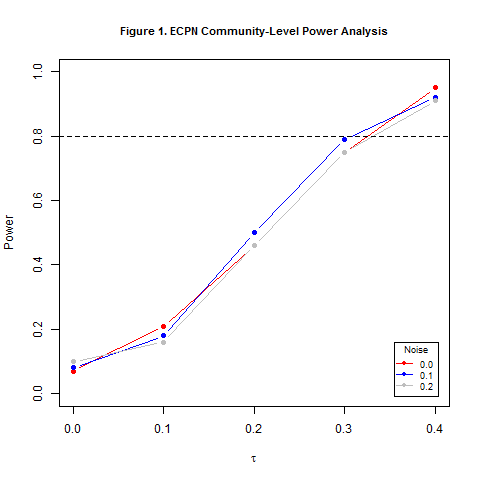
\includegraphics{../../../figures/ecpn_power_figure.png}
\caption{Community-Level Power Analysis}
\end{figure}

Individual-level power analysis suggests we can detect an effect size
between 0.10 = 0.15 SD with a small amount of noise, defined here as
draws from a normal distribution with mean=0 and sd=0.25 SDs. We can
detect an effect size of about 0.20 SD with a moderate amount of noise,
defined here as draws from a normal distribution with mean=0 and sd=0.50
SDs. The power is based on testing 4 hypotheses simultaneously via
Caughey's Non-parametric combinations procedure (Caughey, Dafoe, and
Seawright 2017).

The ``noise'' parameter simulated how much an individual would change
without the ECPN project. Noise at 0.25 SDs translates to an average
change of \textasciitilde1.3 points on a 5 question index where
questions are 4-point Likert scales where options are to (strongly)
agree or (strongly) disagree. Noise at 0.50 SDs translates to an average
change of \textasciitilde2.1 points on the same 5 question index. An
example of a two point change is one respondent moving from ``agree'' to
disagree'' on two of five questions, a respondent moving from ``agree''
to ``strongly agree'' for two of five questions, or a respondent moving
from ``disagree'' to ``strongly agree'' on one question.

\begin{figure}
\centering
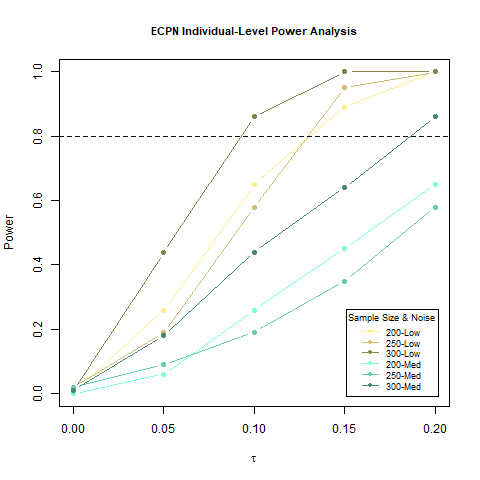
\includegraphics{../../../figures/ecpn_power_figure_ind.png}
\caption{Individual-Level Power Analysis}
\end{figure}

\hypertarget{questions}{%
\section{Survey Question Appendix}\label{questions}}

\textbf{Outgroup Affect}

\begin{itemize}
\tightlist
\item
  With regards to someone from {[}X GROUP{]}, would you feel
  comfortable:

  \begin{itemize}
  \tightlist
  \item
    if they worked in your field?
  \item
    paying them to watch your animals?
  \item
    trading goods with them?
  \item
    sharing a meal with them?
  \item
    with a close relative marrying a person from {[}X GROUP{]}?
  \end{itemize}
\item
  From 1-5, how much do you trust people from {[}X GROUP{]} in your
  area?
\item
  Now I'm going to ask you questions about your community here in
  Benue/Nassarawa, including {[}X GROUP{]}. Please tell me how strongly
  you agree/disagree with each of the following statements: People in
  this area can be trusted.
\end{itemize}

\textbf{Contact}

\begin{itemize}
\tightlist
\item
  Now I'm going to ask you questions about your contact with {[}X
  GROUP{]} in your area.

  \begin{itemize}
  \tightlist
  \item
    Think of the market you go to most frequently. During the past
    month, have members of X GROUP gone to that market too? In the past
    month, how many times did you interact with X group in the market?
  \end{itemize}
\item
  In the past month, have you:

  \begin{itemize}
  \tightlist
  \item
    Joined a member of X group for a social event outside the home? How
    often?
  \item
    Hosted a member of X group for a ceremony in your home? How often?
  \item
    Gone to the home of a member of X group for a ceremony? How often?
  \item
    Have you interacted with members of X group in any other way in the
    past month?
  \end{itemize}
\end{itemize}

\textbf{Insecurity}

\begin{itemize}
\tightlist
\item
  In the last year were there any areas that you avoided going to or
  through because of insecurity during the night?
\item
  In the last year were there any areas that you avoided going to or
  through because of insecurity, during the day?
\item
  In the last year, did insecurity ever prevent you from:

  \begin{itemize}
  \tightlist
  \item
    Working when you wanted to work? About how many days were you unable
    to work?
  \item
    Going to the market?
  \item
    Getting water for the household?
  \item
    Going to your field/farm?
  \item
    Moving your animals to grazing areas?
  \item
    Moving your animals to water?
  \item
    Earning money or going to work?
  \item
    Going to school?
  \end{itemize}
\end{itemize}

\textbf{Endorsement Experiment}

\begin{itemize}
\tightlist
\item
  Imagine that there is a proposal by {[}\textbf{the Farmer's
  Cooperative Society}/\textbf{MACBAN}{]} for action to enhance access
  to clean water in rural areas. Though expensive, the proposal aims to
  bring fresh, clean water to hundreds of areas without access to it,
  including this one. If this were proposed, how would you feel about
  it?
\end{itemize}

\textbf{Percent Experiemnt}

\begin{itemize}
\tightlist
\item
  Think about groups that you might join in your leisure time. Would you
  join a group that had \textbf{5/25/50/75}\% X Group members?
\item
  Think about the community you live in. Would you live in a community
  that had \textbf{5/25/50/75}\% X Group members?
\end{itemize}

\textbf{Violence Placebo}

\begin{itemize}
\tightlist
\item
  Now I am going to ask you some questions about the use of violence. Is
  it always, sometimes, rarely, or never justified to use violence to do
  each of the following:

  \begin{itemize}
  \tightlist
  \item
    Retaliate against violence
  \item
    Defend one's group
  \item
    Maintain culture and traditions
  \item
    Defend one's religion
  \item
    Bring criminals to justice
  \item
    Force the government to change their policies
  \end{itemize}
\end{itemize}

\textbf{Public Goods Game}

``Thank you very much for participating in our survey. Before I go,
there is one last thing. As you may have heard, we have development
funds to use in this community. We have randomly selected you as one of
the 50 people to receive these funds. These funds are not for a Mercy
Corps project, but rather for you to keep personally or to donate to a
community fund.

We have 1,000 Naira to give to you. It is yours, and you can use it
either way--for yourself or for a community good.

Your community and {[}joint farmer/pastoralist community{]} have created
a project committee to whom you can donate this money so that it may be
used to help both communities. The project committee has 4 people from
each community. We have found a donor that will match the funds that you
all contribute to the project committee, so that if you donate 100 Naira
the project committee receives 300 Naira, and if you donate all 1,000
Naira the project committee receives 3,000 Naira. You are welcome to
donate none, some, or all of the money to the project committee.

These are your individual donation envelopes. All the donations will be
private -- only you will know how much money you donated. It essential
that you keep how much you give private -- please do not tell anyone. I
have with me a donation envelope to collect donations. Please go into
your home, put however much of the 1,000 Naira you wish to donate to the
project committee in the envelope, take whatever amount you want to keep
for yourself, and come back to place your envelope in the donation
envelope. Remember, you are welcome to donate none, some, or all of the
money to the project committee. After that we are finished and you may
continue your day. We will come back and publicly announce how much
money your community's project committee will receive.''

\hypertarget{references}{%
\section*{References}\label{references}}
\addcontentsline{toc}{section}{References}

\hypertarget{refs}{}
\begin{CSLReferences}{1}{0}
\leavevmode\vadjust pre{\hypertarget{ref-Caughey2017npc}{}}%
Caughey, Devin, Allan Dafoe, and Jason Seawright. 2017. {``Nonparametric
Combination (NPC): A Framework for Testing Elaborate Theories.''}
\emph{The Journal of Politics} 79 (2): 000--000.

\leavevmode\vadjust pre{\hypertarget{ref-chase2005social}{}}%
Chase, Robert, Michael Woolcock, et al. 2005. {``Social Capital and the
Micro-Institutional Foundations of CDD Approaches in East Asia:
Evidence, Theory, and Policy Implications.''} In \emph{Arusha Conference
{``New Frontiers of Social Policy,''} December}, 12--15.

\leavevmode\vadjust pre{\hypertarget{ref-cilliers2012white}{}}%
Cilliers, Jacobus, Oeindrila Dube, and Bilal Siddiqi. 2012. {``{`White
Man's Burden'}? A Field Experiment on Generosity and Foreigner
Presence.''} In \emph{Paper Presented at the Berkeley Symposium on
Economic Experiments in Developing Countries (SEEDEC)}.

\leavevmode\vadjust pre{\hypertarget{ref-fearon2009can}{}}%
Fearon, James D, Macartan Humphreys, and Jeremy M Weinstein. 2009.
{``Can Development Aid Contribute to Social Cohesion After Civil War?
Evidence from a Field Experiment in Post-Conflict Liberia.''} \emph{The
American Economic Review} 99 (2): 287--91.

\leavevmode\vadjust pre{\hypertarget{ref-galizzi2017external}{}}%
Galizzi, Matteo M, and Daniel Navarro-Martı́nez. 2017. {``On the External
Validity of Social Preference Games: A Systematic Lab-Field Study.''}
\emph{Management Science}.

\leavevmode\vadjust pre{\hypertarget{ref-grossman2012impact}{}}%
Grossman, Guy, and Delia Baldassarri. 2012. {``The Impact of Elections
on Cooperation: Evidence from a Lab-in-the-Field Experiment in
Uganda.''} \emph{American Journal of Political Science} 56 (4): 964--85.

\leavevmode\vadjust pre{\hypertarget{ref-harrison2004field}{}}%
Harrison, Glenn W, and John A List. 2004. {``Field Experiments.''}
\emph{Journal of Economic Literature} 42 (4): 1009--55.

\leavevmode\vadjust pre{\hypertarget{ref-king2013critical}{}}%
King, Elisabeth. 2013. {``A Critical Review of Community-Driven
Development Programmes in Conflict-Affected Contexts.''} \emph{Report
Submitted to International Rescue Committee and UK-Aid}.

\leavevmode\vadjust pre{\hypertarget{ref-paluck2009jsp}{}}%
Paluck, Elizabeth Levy. 2009. {``Reducing Intergroup Prejudice and
Conflict Using the Media: A Field Experiment in Rwanda.''} \emph{Journal
of Personality and Social Psychology} 96 (3): 574.

\leavevmode\vadjust pre{\hypertarget{ref-Paluck2009prejReduction}{}}%
Paluck, Elizabeth Levy, and Donald P Green. 2009. {``Prejudice
Reduction: What Works? A Review and Assessment of Research and
Practice.''} \emph{Annual Review of Psychology} 60: 339--67.

\leavevmode\vadjust pre{\hypertarget{ref-paluck2019contact}{}}%
Paluck, Elizabeth Levy, Seth A Green, and Donald P Green. 2019. {``The
Contact Hypothesis Re-Evaluated.''} \emph{Behavioural Public Policy} 3
(2): 129--58.

\leavevmode\vadjust pre{\hypertarget{ref-pettigrew2006meta}{}}%
Pettigrew, Thomas F, and Linda R Tropp. 2006. {``A Meta-Analytic Test of
Intergroup Contact Theory.''} \emph{Journal of Personality and Social
Psychology} 90 (5): 751.

\leavevmode\vadjust pre{\hypertarget{ref-scacco2018nigeria}{}}%
Scacco, Alexandra, and Shana S Warren. 2018. {``Can Social Contact
Reduce Prejudice and Discrimination? Evidence from a Field Experiment in
Nigeria.''} \emph{American Political Science Review} 112 (3): 654--77.

\leavevmode\vadjust pre{\hypertarget{ref-winking2013natural}{}}%
Winking, Jeffrey, and Nicholas Mizer. 2013. {``Natural-Field Dictator
Game Shows No Altruistic Giving.''} \emph{Evolution and Human Behavior}
34 (4): 288--93.

\end{CSLReferences}

\end{document}
